\documentclass{beamer}
%
% Choose how your presentation looks.
%
% For more themes, color themes and font themes, see:
% http://deic.uab.es/~iblanes/beamer_gallery/index_by_theme.html
%
\mode<presentation>
{
  \usetheme{Madrid}      % or try Darmstadt, Madrid, Warsaw, ...
  \usecolortheme{beaver} % or try albatross, beaver, crane, ...
  \usefonttheme{serif}  % or try serif, structurebold, ...
  \setbeamertemplate{navigation symbols}{}
  \setbeamertemplate{caption}[numbered]
} 

\usepackage{hyperref}
\usepackage[english]{babel}
\usepackage[utf8x]{inputenc}
\usepackage{pdfpages}
\usepackage{framed, color}
\definecolor{shadecolor}{rgb}{1,0.8,0.3}
\usepackage{color}
 
\definecolor{codegreen}{rgb}{0,0.6,0}
\definecolor{codegray}{rgb}{0.5,0.5,0.5}
\definecolor{codepurple}{rgb}{0.58,0,0.82}
\definecolor{backcolour}{rgb}{0.95,0.95,0.92}
\definecolor{pblue}{rgb}{0.13,0.13,1}
\definecolor{pgreen}{rgb}{0,0.5,0}
\definecolor{pred}{rgb}{0.9,0,0}
\definecolor{pgrey}{rgb}{0.46,0.45,0.48}
 
\usepackage{listings}
\lstset{language=Python,
  showspaces=false,
  showtabs=false,
  breaklines=true,
  showstringspaces=false,
  breakatwhitespace=true,
  commentstyle=\color{pgreen},
  keywordstyle=\color{pblue},
  stringstyle=\color{pred},
  basicstyle=\ttfamily,
  frame=lrbt,xleftmargin=\fboxsep,xrightmargin=-\fboxsep
}

\title[Ragazze Digitali 2019]{Ragazze Digitali A.A. 2018/2019}
\author{E. Salvucci - S. Gattucci - C. Varini}
\date{}

\AtBeginSection[]
{
  \begin{frame}<beamer>
    \frametitle{Outline}
    \tableofcontents[currentsection,currentsubsection]
  \end{frame}
}

\begin{document}

\setbeamertemplate{background}
{
\includegraphics[width=\paperwidth,height=\paperheight]{images/ragazze_digitali.jpg}}
\begin{frame}
\end{frame}

\setbeamertemplate{background}
% Python

\begin{frame}{Cosa faremo oggi}
    \vspace{0.8cm}
      Impareremo ad usare \texttt{pygame}, un modulo che permette di creare giochi completi di animazioni, suoni e comandi con il mouse.
\end{frame}

\section{Installare pygame}

\begin{frame}[fragile]
\frametitle{Installare pygame su Spyder}
	\begin{block}{Come installare \texttt{pygame}}
		\begin{itemize}
			\item Per installare pygame su Spyder è sufficiente andare su \textit{\textbf{Start $>$ anaconda3 $>$ anaconda prompt}} e digitare nella finestra che appare il comando \texttt{pip install pygame}
			\item Per controllare se è stato correttamente installato scriviamo sulla shell di Python il comando \texttt{import pygame} e verifichiamo che l'output sia simile a quello in figura:
			\begin{figure}[t]
				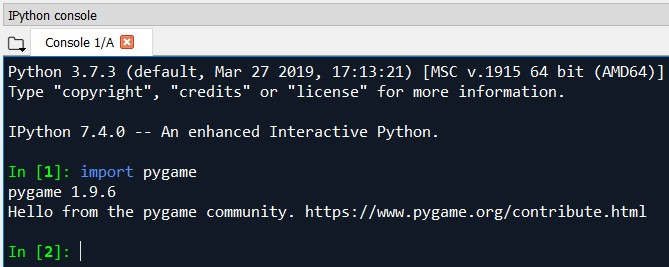
\includegraphics[height=2.9cm, width=9cm]{images/Import-pygame.jpg}
			\end{figure}
			\item Sui pc della scuola è già installato, quindi ora iniziamo a vedere qualche comando!
		\end{itemize}
	\end{block}
\end{frame}

\begin{frame}[fragile]
\frametitle{Installare pygame su PyCharm 1/2}
\begin{block}{Come installare \texttt{pygame}}
	\begin{itemize}
		\item Per installare pygame su PyCharm è sufficiente aprire il progetto corrente, andare su \textbf{File $>$ Settings $>$ Project: $>$ Project Interpreter} (come cerchiato in figura a sinistra); a questo punto, cliccare il pulsante "+" a destra (cerchiato in figura), cercare nella barra in alto \textit{"pygame"}, selezionarlo e cliccare \textit{"Install Package"}
		\begin{figure}[t]
			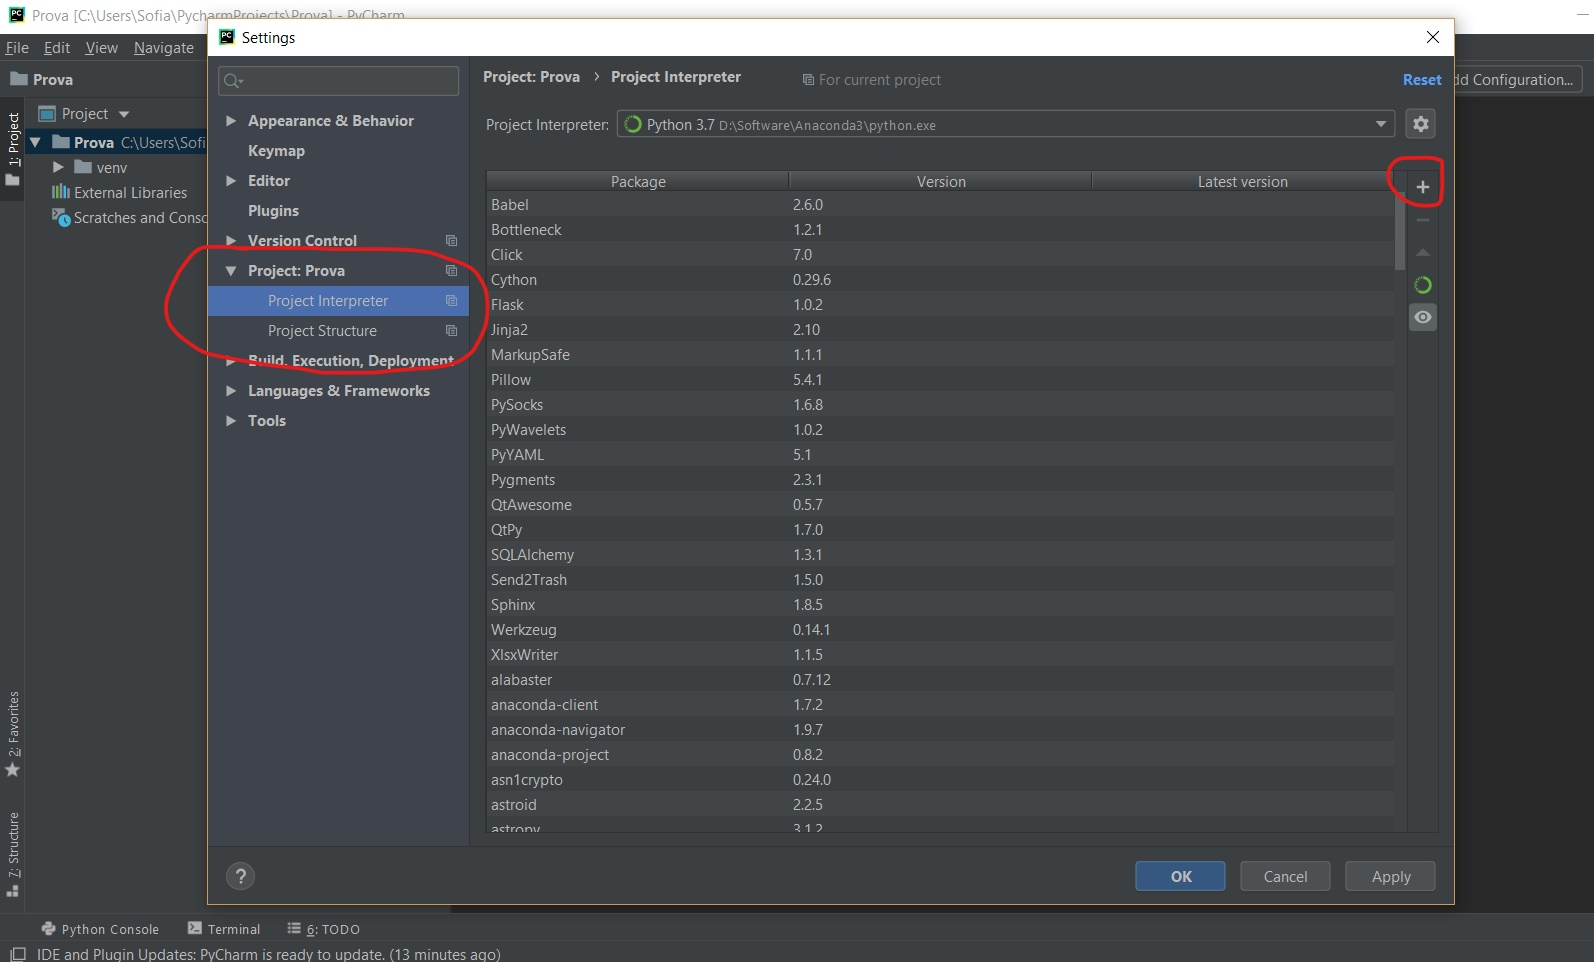
\includegraphics[height=4.5cm, width=9cm]{images/PyCharm.jpg}
		\end{figure}
	\end{itemize}
\end{block}
\end{frame}

\begin{frame}[fragile]
\frametitle{Installare pygame su PyCharm 2/2}

Per controllare se è stato correttamente installato, creiamo un file all'interno del progetto, scriviamo queste due righe di codice ed eseguiamo.
\begin{lstlisting}
import pygame
pygame.init()
		\end{lstlisting}
		\begin{figure}[t]
			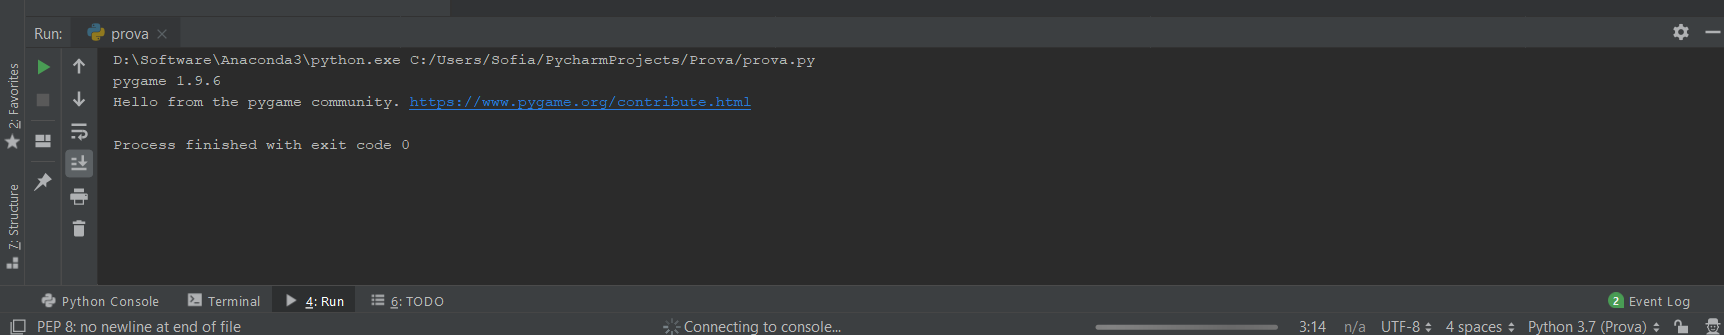
\includegraphics[height=2.9cm, width=11cm]{images/PyCharmOK.png}
		\end{figure}
Sui pc della scuola è già installato, quindi ora iniziamo a vedere qualche comando!

\end{frame}

\section{Primi comandi}

\begin{frame}[fragile]
\frametitle{Import e impostazione della finestra}
	Innanzitutto importiamo e inizializziamo il modulo \texttt{pygame} nel nostro programma con queste semplici istruzioni:
	\begin{columns}[T]
		\begin{column}[T]{0.55\textwidth}
	\begin{lstlisting}
import pygame, sys
from pygame.locals import *

pygame.init()
	\end{lstlisting}
		\end{column}
\begin{column}[T]{0.45\textwidth}
	\begin{figure}[t]
		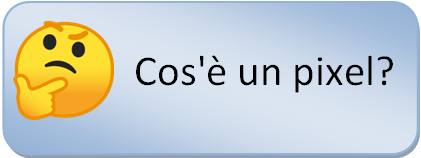
\includegraphics[height=2cm, width=5cm]{images/CosaPixel.png}
	\end{figure}
\end{column}
\end{columns}
	Per impostare la finestra che utilizzeremo il metodo \texttt{set\_mode()} del modulo \texttt{display}, al quale ci si accede dal modulo \texttt{pygame}
\begin{lstlisting}
windowSurface = pygame.display.set_mode((500, 400), 0, 32)
\end{lstlisting}
In questo modo, viene impostata una finestra larga \textbf{500} pixel e alta \textbf{400} pixel. Gli altri due parametri (0 e 32), per questo corso, li copiamo senza approfondire.
\end{frame}

\begin{frame}[fragile]
\frametitle{Import e impostazione della finestra}
Innanzitutto importiamo e inizializziamo il modulo \texttt{pygame} nel nostro programma con queste semplici istruzioni:
\begin{columns}[T]
	\begin{column}[T]{0.55\textwidth}
		\begin{lstlisting}
import pygame, sys
from pygame.locals import *
		
pygame.init()
		\end{lstlisting}
	\end{column}
	\begin{column}[T]{0.45\textwidth}
		\begin{figure}[t]
			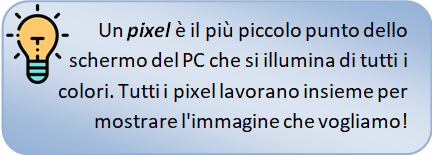
\includegraphics[height=2cm, width=5cm]{images/pixel.png}
		\end{figure}
	\end{column}
\end{columns}
Per impostare la finestra che utilizzeremo il metodo \texttt{set\_mode()} del modulo \texttt{display}, al quale ci si accede dal modulo \texttt{pygame}
\begin{lstlisting}
windowSurface = pygame.display.set_mode((500, 400), 0, 32)
\end{lstlisting}
In questo modo, viene impostata una finestra larga \textbf{500} pixel e alta \textbf{400} pixel. Gli altri due parametri (0 e 32), per questo corso, li copiamo senza approfondire.
\end{frame}

\section{Tuple e colori}

\begin{frame}[fragile]
\frametitle{Tuple e colori 1/3}
	\begin{block}{Tuple}
		\begin{itemize}
			\item Una tupla è simile ad una lista, con la differenza che si usano le parentesi () al posto che le []. Non possono essere modificate.
		\end{itemize}
	\end{block}
\begin{lstlisting}
>>> spam = ('Life', 'Universe', 'Everything', 42)
>>> spam[0]
>>> spam[3]
>>> spam[3] = 'Hello'
\end{lstlisting}
Eseguiamo, una per volta queste righe e osserviamo il comportamento!\\
All'interno del metodo \texttt{set\_mode()} abbiamo usato una tupla per definire la grandezza della finestra in pixel.\\
Vedremo che ci saranno utili in seguito!
\end{frame}

\begin{frame}[fragile]
\frametitle{Tuple e colori 2/3}
\begin{block}{Colori}
	\begin{itemize}
		\item Ogni pixel viene illuminato da 3 colori primari quali \textbf{rosso}, \textbf{verde} e \textbf{blu} (RGB). Combinando questi tre semplici colori, si è in grado di ottenere qualsiasi altro colore.
		\item In pygame, per definire i colori useremo delle tuple formate dai tre valori (\textbf{R}ed - \textbf{G}reen - \textbf{B}lue)
	\end{itemize}
\end{block}
\begin{columns}[T]
	\begin{column}[T]{0.55\textwidth}
		\begin{lstlisting}
# Set up the colors.
BLACK = (0, 0, 0)
WHITE = (?, ?, ?)
RED = (255, 0, 0)
GREEN = (?, ?, ?)
BLUE = (?, ?, ?)
		\end{lstlisting}
	\end{column}
	\begin{column}[T]{0.45\textwidth}
		\begin{figure}[t]
			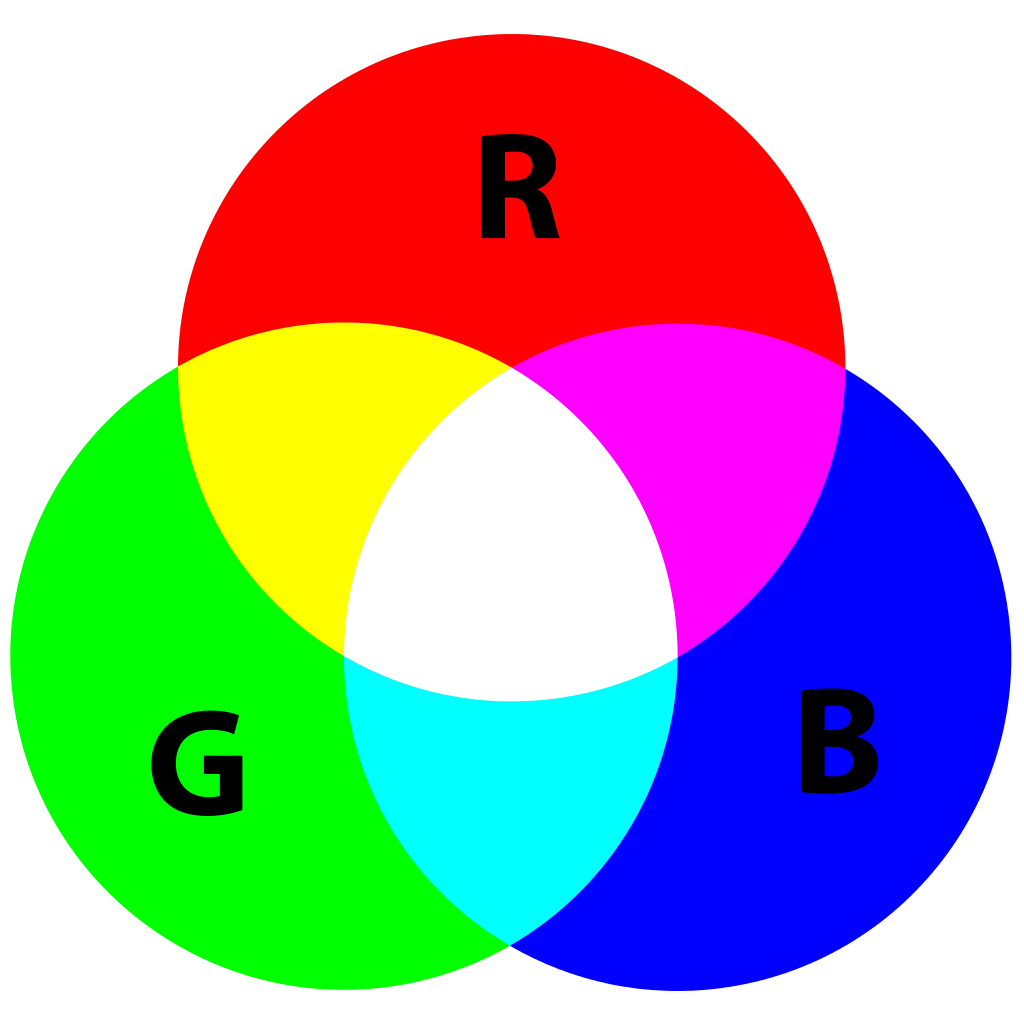
\includegraphics[height=3cm, width=3cm]{images/RGB.png}
		\end{figure}
	\end{column}
\end{columns}
\end{frame}

\begin{frame}[fragile]
\frametitle{Tuple e colori 3/3}
\begin{block}{Colori}
	\begin{itemize}
		\item Ogni numero della tupla rappresenta la "quantità" di ciascun colore, che può andare da 0 a 255.
		\item Il primo numero rappresenta la quantità di rosso, il secondo la quantità di verde e il terzo quella del blu.
	\end{itemize}
\end{block}
\begin{columns}[T]
	\begin{column}[T]{0.5\textwidth}
		\begin{lstlisting}
# Set up the colors.
BLACK = (0, 0, 0)
WHITE = (255, 255, 255)
RED = (255, 0, 0)
GREEN = (0, 255, 0)
BLUE = (0, 0, 255)
		\end{lstlisting}
	\end{column}
	\begin{column}[T]{0.5\textwidth}
		\begin{figure}[t]
			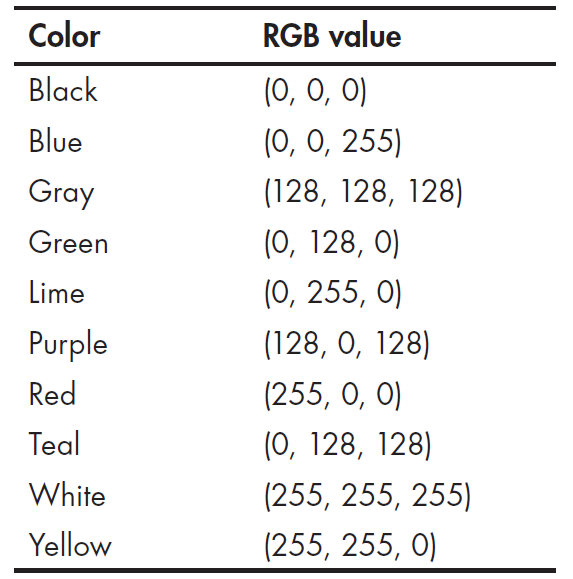
\includegraphics[height=4.5cm, width=6cm]{images/TabellaColori.png}
		\end{figure}
	\end{column}
\end{columns}
\end{frame}

\section{Scrivere testi in pygame}

\begin{frame}[fragile]
\frametitle{Fonts 1/2}
\begin{lstlisting}
# Set up the fonts.
basicFont = pygame.font.SysFont(None, 48)
\end{lstlisting}
\begin{block}{Impostare un font}
	\begin{itemize}
		\item Attraverso la funzione \texttt{pygame.font.SysFont()} è possibile impostare il font del nostro testo.
		\item Questa funzione prende in input due parametri: il primo è il nome del font (in questo caso viene impostato quello di default) e il secondo parametro è la grandezza.
		\item Salviamo il risultato di questa funzione nella variabile \texttt{basicFont}, sulla quale invocheremo il metodo \texttt{render()}
	\end{itemize}
\end{block}
\end{frame}

\begin{frame}[fragile]
\frametitle{Fonts 2/2}
\begin{lstlisting}
# Set up the text.
text = basicFont.render('Hello world!', True, WHITE, BLUE)
\end{lstlisting}

\begin{columns}
	\begin{column}[T]{0.7\textwidth}
		\begin{block}{Impostare un font}
			\begin{itemize}
				\item Questo metodo permette di \textit{renderizzare} la scritta che inseriremo in una variabile \texttt{text}.
				\item Il secondo parametro permette di creare un effetto \textit{"blur"} al testo, chiamato anti-alias, come in figura.
				\item Il terzo e quarto paragrafo indicano il colore del testo e del backgroun, (sfondo), rispettivamente.
			\end{itemize}
		\end{block}
	\end{column}
	\begin{column}[T]{0.3\textwidth}
		\begin{figure}[t]
			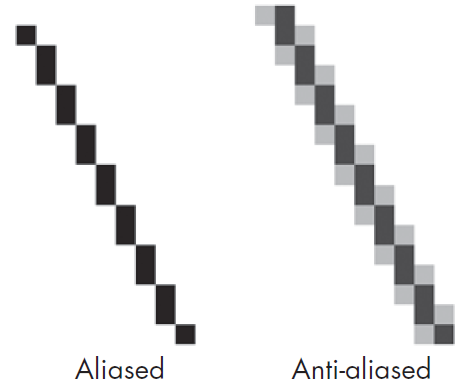
\includegraphics[height=2.5cm, width=2.5cm]{images/anti-aliased.png}
		\end{figure}
	\end{column}
\end{columns}

\end{frame}


\begin{frame}[fragile]
\frametitle{Come disporre un testo nella finestra}
\begin{lstlisting}
textRect = text.get_rect()
textRect.centerx = windowSurface.get_rect().centerx
textRect.centery = windowSurface.get_rect().centery
\end{lstlisting}

	\begin{block}{Disposizione testo}
		\begin{itemize}
			\item Il metodo \texttt{get\_rect()} serve per disporre il nostro testo all'interno della finestra.
			\item Ciò che otteniamo con l'invocazione di questo metodo lo possiamo inserire all'interno di una variabile (\texttt{textRect}), e su di essa possiamo accedere ad alcuni valori che ci danno informazioni utili per capire e impostare la posizione del testo.
		\end{itemize}
	\end{block}
\end{frame}

\begin{frame}[fragile]
\frametitle{Tabella di attributi Rect object}
\begin{columns}
	\begin{column}[T]{0.7\textwidth}
		\begin{figure}[t]
			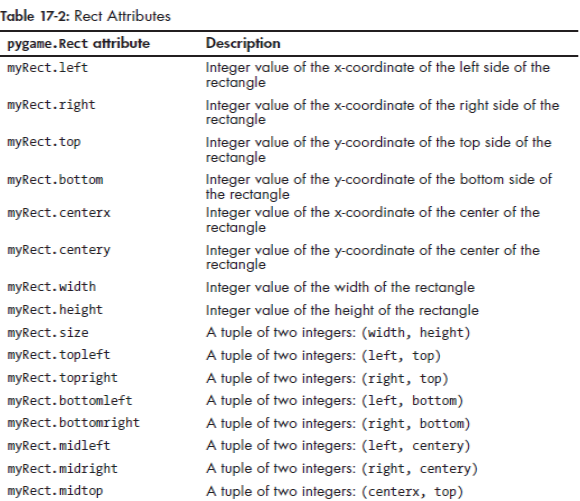
\includegraphics[height=7cm, width=7cm]{images/attributiRect.png}
		\end{figure}
	\end{column}
	\begin{column}[T]{0.3\textwidth}
		Ecco alcuni valori a cui possiamo accedere e che potranno esserci utili in futuro.\\
		
	\end{column}
\end{columns}
\end{frame}

\section{Disegnare con pygame}

\begin{frame}[fragile]
\frametitle{Colorare un oggetto}
\begin{block}{fill()}
	\begin{itemize}
		\item E' possibile riempire un oggetto di colore tramite il metodo \texttt{fill()}.
		\item Questa funzione prende in ingresso una tupla che rappresenta un colore.
		\item Nel nostro esempio, abbiamo usato questa funzione per impostare lo sfondo della finestra.
	\end{itemize}
\end{block}
\begin{lstlisting}
# Draw the white background onto the surface.
windowSurface.fill(WHITE)
\end{lstlisting}
\end{frame}

\begin{frame}[fragile]
\frametitle{Disegnare un poligono}
\begin{block}{polygon()}
	Questa funzione permette di creare qualsiasi tipo di poligono. Vediamone gli argomenti in input:
	\begin{itemize}
		\item la finestra su cui disegnare il poligono;
		\item il colore;
		\item una tupla di n tuple (coppie di valori x,y) che indicano i punti del poligono. L'ultimo punto si collegherà automaticamente al primo;
		\item un intero, opzionale, che determina lo spessore del contorno. Senza di esso, il poligono è riempito.
	\end{itemize}
\end{block}
\begin{lstlisting}
# Draw a green polygon onto the surface.
pygame.draw.polygon(windowSurface, GREEN, ((146, 0), (291, 106),
(236, 277), (56, 277), (0, 106)))
\end{lstlisting}
\end{frame}


\begin{frame}[fragile]
\frametitle{Disegnare una linea}
\begin{block}{line()}
	Questa funzione permette di creare una linea. Vediamone gli argomenti in input:
	\begin{itemize}
		\item la finestra su cui disegnare la linea;
		\item il colore;
		\item una tupla di valori x,y che indica un capo della linea;
		\item una tupla di valori x,y che indica l'altro capo della linea;
		\item un intero, opzionale, che indica lo spessore della linea
	\end{itemize}
\end{block}
\begin{lstlisting}
pygame.draw.line(windowSurface, BLUE, (60, 60), (120, 60), 4)
pygame.draw.line(windowSurface, BLUE, (120, 60), (60, 120))

\end{lstlisting}
\end{frame}


\begin{frame}[fragile]
\frametitle{Disegnare un cerchio}
\begin{block}{circle()}
	Questa funzione permette di creare un cerchio. Vediamone gli argomenti in input:
	\begin{itemize}
		\item la finestra su cui disegnare il cerchio;
		\item il colore;
		\item una tupla di valori x,y che indica il centro del cerchio;
		\item un intero che indica il raggio;
		\item un intero, opzionale, che indica lo spessore della linea. Se è 0, il cerchio viene riempito.
	\end{itemize}
\end{block}
\begin{lstlisting}
# Draw a blue circle onto the surface.
pygame.draw.circle(windowSurface, BLUE, (300, 50), 20, 0)

\end{lstlisting}
\end{frame}

\begin{frame}[fragile]
\frametitle{Disegnare un ellisse}
\begin{block}{ellipse()}
	Questa funzione permette di creare un ellisse. Vediamone gli argomenti in input:
	\begin{itemize}
		\item la finestra su cui disegnare l'ellisse;
		\item il colore;
		\item una tupla contenente l'angolo di sinistra e in alto, la larghezza e l'altezza dell'ellisse;
		\item un intero, opzionale, che indica lo spessore della linea. Se è 0, l'ellisse viene riempito.
	\end{itemize}
\end{block}
\begin{lstlisting}
# Draw a red ellipse onto the surface.
pygame.draw.ellipse(windowSurface, RED, (300, 250, 40, 80), 1)

\end{lstlisting}
\end{frame}

\begin{frame}[fragile]
\frametitle{Disegnare un rettangolo}
\begin{block}{circle()}
	Questa funzione permette di creare un cerchio. Vediamone gli argomenti in input:
	\begin{itemize}
		\item la finestra su cui disegnare il cerchio;
		\item il colore;
		\item una tupla con 4 valori, rispettivamente le coordinate x,y per gli spigoli alto-sinistra, larghezza e altezza 
	\end{itemize}
\end{block}
\begin{lstlisting}
pygame.draw.rect(windowSurface, RED, (textRect.left - 20,
textRect.top - 20, textRect.width + 40, textRect.height + 40))

\end{lstlisting}
\end{frame}

\begin{frame}[fragile]
\frametitle{Disegnare una finestra dentro l'altra}
\begin{block}{blit()}
	Questo metodo permette di disegnare due finestre, una dentro l'altra. Nel nostro esempio, infatti, abbiamo la finestra contenente la scritta e la finestra contenente le figure. Vediamo come sovrappporle.
\end{block}
\begin{lstlisting}
# Draw the text onto the surface.
windowSurface.blit(text, textRect)
\end{lstlisting}
In questo caso, la finestra contenente la scritta viene inserita all'interno della finestra con le figure.\\
Facciamo bene attenzione quindi all'ordine con cui sovrapponiamo le due finestre!
\end{frame}

\section{Display e Game loop}

\begin{frame}[fragile]
\frametitle{Stampare a schermo le nostre creazioni}
\begin{lstlisting}
# Draw the window onto the screen.
pygame.display.update()
\end{lstlisting}
Con questo semplice metodo riusciamo a rendere visibile sul nostro display tutto ciò che abbiamo creato fino ad ora!
\end{frame}

\begin{frame}[fragile]
\frametitle{Eventi e game loop}
\begin{block}{Eventi}
	\begin{itemize}
		\item Un evento è qualcosa che accade all'interno del nostro programma, come un click o movimento del mouse o la pressione di un tasto.
		\item Possiamo intercettare gli eventi tramite la funzione \texttt{get()}, mentre il valore \texttt{type} (a cui accediamo tramite \texttt{event.type}) indica il tipo di evento di cui si tratta.
		\item L'\texttt{if} contenuto nel game loop intercetta l'evento di uscita e se si verifica, vengono invocati i metodi \texttt{pygame.quit()} e \texttt{sys.exit()}.
	\end{itemize}
\end{block}
\begin{lstlisting}
# Run the game loop.
while True:
    for event in pygame.event.get():
        if event.type == QUIT:
            pygame.quit()
            sys.exit()
\end{lstlisting}
\end{frame}

\section{Primo giochino con animazioni}

\begin{frame}[fragile]
\frametitle{Animazioni}
Costruiremo un programma nel quale 3 quadrati colorati diversamente che si muoveranno all'interno della finestra. Ogni quadratino si muoverà in diagonale in una delle 4 direzioni. Se si scontra con un bordo della finestra, rimbalzerà in un'altra direzione, come mostrato in figura sotto.
\begin{columns}
	\begin{column}[T]{0.5\textwidth}
		\begin{figure}[t]
			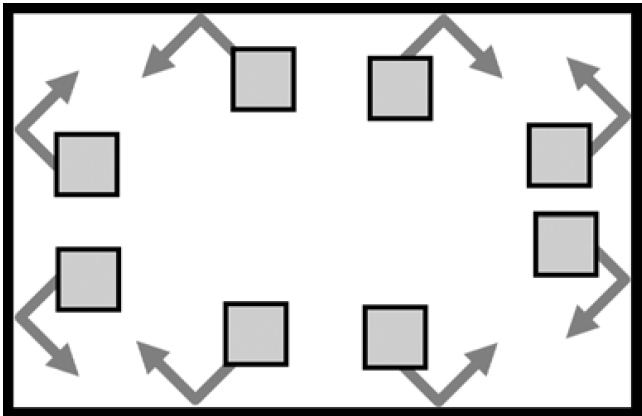
\includegraphics[height=3cm, width=4cm]{images/animazioni.png}
		\end{figure}
	\end{column}
	\begin{column}[T]{0.5\textwidth}
		\begin{itemize}
			\item In quale direzione si muoverà il quadratino? Da cosa dipende?
		\end{itemize}
	\end{column}
\end{columns}
\end{frame}

\begin{frame}[fragile]
\frametitle{Animazioni}
Costruiremo un programma nel quale 3 quadrati colorati diversamente che si muoveranno all'interno della finestra. Ogni quadratino si muoverà in diagonale in una delle 4 direzioni. Se si scontra con un bordo della finestra, rimbalzerà in un'altra direzione, come mostrato in figura sotto.
\begin{columns}
	\begin{column}[T]{0.5\textwidth}
		\begin{figure}[t]
			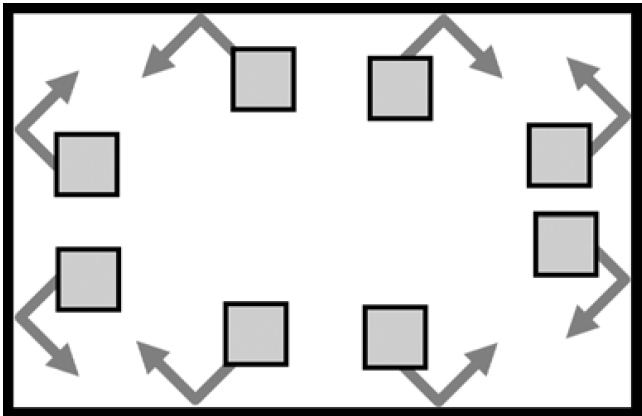
\includegraphics[height=3cm, width=4cm]{images/animazioni.png}
		\end{figure}
	\end{column}
	\begin{column}[T]{0.5\textwidth}
		\begin{itemize}
			\item In quale direzione si muoverà il quadratino? Da cosa dipende?
			\textbf{1)} Dalla direzione in cui si muoveva prima di rimbalzare; \\
			\textbf{2)} In che muro ha rimbalzato.
		\end{itemize}
	\end{column}
\end{columns}
\end{frame}

\begin{frame}[fragile]
\frametitle{Setting delle costanti delle figure}
\lstset{basicstyle=\tiny}
	\begin{lstlisting}
import pygame, sys, time
from pygame.locals import *
# Set up pygame.
pygame.init()
# Set up the window.
WINDOWWIDTH = 400
WINDOWHEIGHT = 400
windowSurface = pygame.display.set_mode((WINDOWWIDTH, WINDOWHEIGHT), 0, 32)
pygame.display.set_caption('Animation')
# Set up direction variables.
DOWNLEFT = 'downleft'
DOWNRIGHT = 'downright'
UPLEFT = 'upleft'
UPRIGHT = 'upright'
MOVESPEED = 4
# Set up the colors.
WHITE = (?, ?, ?)
RED = (?, ?, ?)
GREEN = (?, ?, ?)
BLUE = (?, ?, ?)

# Set up the box data structure.
b1 = {'rect':pygame.Rect(300, 80, 50, 100), 'color':RED, 'dir':UPRIGHT}
b2 = {'rect':pygame.Rect(200, 200, 20, 20), 'color':GREEN, 'dir':UPLEFT}
b3 = {'rect':pygame.Rect(100, 150, 60, 60), 'color':BLUE, 'dir':DOWNLEFT}
boxes = [b1, b2, b3]
	\end{lstlisting}
\end{frame}


\begin{frame}[fragile]
\frametitle{Game Loop 1/3}
\lstset{basicstyle=\tiny}
\begin{columns}
	\begin{column}[T]{0.5\textwidth}
		\begin{lstlisting}
while True:
    # Check for the QUIT event.
    for ? in ?:
		?
		
    # Draw the white background onto the surface.
    windowSurface.fill(WHITE)
    
    for b in boxes:
    # Move the box data structure.
        if ? == ?:
            ?
        if ? == ?:
            ?
        if ? == ?:
            ?
        if ? == ?:
            ?
		
		\end{lstlisting}
	\end{column}
	\begin{column}[T]{0.5\textwidth}
		All'interno del secondo \texttt{for}, inseriamo una serie di controlli che permettono alle figure di muoversi.\\
		\begin{itemize}
		\item \textbf{SE} la direzione è \texttt{DOWNLEFT} o \texttt{DOWNRIGHT}, va \textit{incrementato} l'attributo \texttt{top};
		\item \textbf{SE} la direzione è \texttt{UPLEFT} o \texttt{UPRIGHT,}, va \textit{decrementato} l'attributo \texttt{top};
		\item \textbf{SE} la direzione è \texttt{DOWNRIGHT} o \texttt{UPRIGHT,}, va \textit{incrementato} l'attributo \texttt{lef};
		\item \textbf{SE} la direzione è \texttt{DOWNLEFT} o \texttt{UPLEFT,}, va \textit{decrementato} l'attributo \texttt{left};
		\end{itemize}
		
	\end{column}
\end{columns}
\end{frame}

\begin{frame}[fragile]
\frametitle{Game Loop 2/3}
\lstset{basicstyle=\tiny}
\begin{columns}
	\begin{column}[T]{0.5\textwidth}
		\begin{lstlisting}
        if b['rect'].top < 0:
            # The box has moved past the top.
            ?
		
        if b['rect'].bottom > WINDOWHEIGHT:
            # The box has moved past the bottom.
            ?
		
        if b['rect'].left < 0:
            # The box has moved past the left side.
            ?
		
        if b['rect'].right > WINDOWWIDTH:
            # The box has moved past the right side.
            ?
		
		\end{lstlisting}
	\end{column}
	\begin{column}[T]{0.5\textwidth}
		Sempre all'interno del secondo \texttt{for}, inseriamo una serie di controlli che permettono alle figure di "rimbalzare" nel caso in cui si scontrino con il bordo.\\
		\begin{itemize}
			\item \textbf{SE} ha toccato il bordo superiore, se era \texttt{UPLEFT} o \texttt{UPRIGHT}, diventerò \texttt{DOWNLEFT} o \texttt{DOWNRIGHT}
			\item \textbf{SE} ha toccato quello inferiore, \texttt{UPLEFT} o \texttt{UPRIGHT} diventeranno \texttt{UPLEFT} o \texttt{UPRIGHT}
			\item \textbf{SE} ha toccato quello destro, cosa succederà? E quello sinistro?
		\end{itemize}
		
	\end{column}
\end{columns}
\end{frame}


\begin{frame}[fragile]
\frametitle{Game Loop 3/3}
		\begin{lstlisting}
        # Draw the box onto the surface.
        pygame.draw.rect(windowSurface, b['color'], b['rect'])
		
    # Draw the window onto the screen.
    pygame.display.update()
    time.sleep(0.02)
		\end{lstlisting}
		Ultime righe di questo codice che permettono di disegnare ogni rettangolo nella nuova posizione. \\Occhio che questa la prima funzione è inserita nel \texttt{for}, mentre le ultime due sono fuori dal \texttt{for} ma sempre dentro il game loop.\\
		La funzione \texttt{display.update()} serve per aggiornare la nostra finestra, in modo che sia visibile lo spostamento delle figure!
\end{frame}


\begin{frame}

\begin{center}
	\bigskip
	Materiale rilasciato con licenza
	
	\textbf{\href{http://creativecommons.org/licenses/by-sa/4.0/}{Creative Commons - Attributions, Share-alike 4.0}}
	
	\medskip
	
\includegraphics[height=0.8cm]{images/cc.jpeg}
\end{center}

\end{frame}
	
\end{document}